%\documentclass[11pt,a4paper,uplatex,dvipdfmx]{ujarticle} 		% for uplatex
\documentclass[11pt,a4j,dvipdfmx]{jarticle} 					% for platex
\input{pieces/form00_header} % pieces
\input{pieces/kakenhi7} % pieces
% form01_header.tex
% 2017-05-28 Split from form00_header.tex to move \input{kakenhiLaTeX7.sty} to mother_1.tex.
% 2010-01-15 Adjusted margins.
% ===== Parameters for KL (Kakenhi LaTeX) ========================
%%\geometry{noheadfoot,scale=1}  %scale=1 resets margins to 0
\setlength{\unitlength}{1pt}

\newlength{\KLCella}
\newlength{\KLCellb}
\newlength{\KLCellc}
\newlength{\KLCelld}
\newlength{\KLCelle}
\newlength{\KLCellf}

\newcounter{KLMaxYearCount}	% # of years for the proposal
\newcommand{\KLCLLang}{}	% language-dependent left-justification in tabular

% ===== format and header =========
% 2020-01-15: Reset it to match the margins (25 mm on sides, 20 mm on top and bottom). 
% A4: 294 mm x 210 mm.  
% LaTeX's default margin is 1 inch = 25.4 mm.
\setlength{\oddsidemargin}{-1pt}	% (25.0 - 25.4) / 25.4 * 72 pt/inch = -1 pt
\setlength{\evensidemargin}{-1pt}
\setlength{\textwidth}{453pt}		% (210 - 25*2) / 25.4 * 72 = 453 pt
\setlength{\topmargin}{-61pt}	% This and \headheight determine the actual top margin
\setlength{\textheight}{254mm}		% (294 - 20*2) = 254 mm

\setlength{\headheight}{48pt}
\setlength{\headsep}{3pt}

\cfoot{}
\renewcommand{\headrulewidth}{0pt}

\pagestyle{empty}
% ==== other applications table =========
\newcommand{\KLTableHeaderFont}{\fontsize{8.2}{11}\selectfont}
\newcommand{\KLTableHeaderSmallFont}{\fontsize{7.5}{10}\selectfont}
\newcommand{\KLTableHeaderSmallerFont}{\fontsize{7}{10}\selectfont}

 % pieces
% ===== Global year-dependent definitions for the Kakenhi form ===========
% 基本情報
\newcommand{\研究開始年度}{2022}
\newcommand{\研究開始元号年度}{04}	%令和

\newcommand{\一年目西暦}{2022}
\newcommand{\二年目西暦}{2023}
\newcommand{\三年目西暦}{2024}
\newcommand{\四年目西暦}{2025}
\newcommand{\五年目西暦}{2026}
\newcommand{\六年目西暦}{2027}

\newcommand{\一年目}{4}
\newcommand{\二年目}{5}
\newcommand{\三年目}{6}
\newcommand{\四年目}{7}
\newcommand{\五年目}{8}
\newcommand{\六年目}{9}

\newcommand{\一年目J}{4}
\newcommand{\二年目J}{5}
\newcommand{\三年目J}{6}
\newcommand{\四年目J}{7}
\newcommand{\五年目J}{8}
\newcommand{\六年目J}{9}


 % pieces
\input{pieces/hook3} % pieces
%#Name: chousenteki_houga
% form04_jsps_headers.tex
% 2017-08-20 Taku
% 2017-08-29 Taku
%			Added a check against jsps-abs-p1-header.
% 2017-09-02 Taku
%			Added sectionNo to the commands to make them compatible with 
%			\KLBeginSubjectWithHeaderCommands.
%			Use \KLJInt.
% 2018-09-01 Taku
%			Adjusted the heights of the headers by inserting \vspace{-3pt} and \rule.
%
\newcommand{\headerfont}{\fontsize{11}{11}\selectfont}
% ===== Headers =====================================
\newcommand{\JSPSVeryFirstPageStyle}[5]{%
%	Defines the header for the very first page of the form.
%	Called from \KLShumokuFirstPageStyle in form04_***.
%--------------------------------
%	#1: page style name
%	#2: 様式
%	#3: 研究種目名
%	#4: 項目名
%	#5: sectionNo
%--------------------------------
	\fancypagestyle{JSPSVeryFirstPageStyle}{% The name is not taken from #1, because 
		\fancyhf{}
		\fancyhead[L]{\hspace{-37pt}\headerfont#2\ 研究計画調書(添付ファイル項目)\\
				\rule{0pt}{18pt}\\}
%				\rule{0pt}{0pt}\\}
		\fancyhead[R]{\headerfont\textbf{#3\ \KLJInt{\thepage}}\vspace{-5pt}\\
			\rule{0pt}{0pt}\\}
%		\fancyhead[R]{\headerfont\textbf{#3\ \KLJInt{\thepage}\\}}
	}
	\thispagestyle{JSPSVeryFirstPageStyle}
}

\newcommand{\JSPSFirstSubjectPageStyle}[5]{%
%	Defines the header for the first page for the subject.
%	Called from \KLShumokuFirstPageStyle in form04_***.
%--------------------------------
%	#1: page style name
%	#2: 様式
%	#3: 研究種目名
%	#4: 項目名
%	#5: sectionNo
%--------------------------------
	\fancypagestyle{JSPSFirstSubjectPageStyle}{%
		\fancyhf{}
		\fancyhead[R]{\headerfont\textbf{#3\ \KLJInt{\thepage}}\vspace{-5pt}\\
			\rule{0pt}{0pt}\\}
%		\fancyhead[R]{\headerfont\textbf{#3\ \KLJInt{\thepage}\\}}
	}
	\thispagestyle{JSPSFirstSubjectPageStyle}
}

\newcommand{\JSPSDefaultPageStyle}[5]{%
%	Defines the default header for the subject.
%	Called from \KLShumokuDefaultPageStyle in form04_***.
%--------------------------------
%	#1: page style name
%	#2: 様式
%	#3: 研究種目名
%	#4: 項目名
%	#5: sectionNo
%--------------------------------
	\fancypagestyle{JSPSDefaultPageStyle}{%
		\fancyhf{}
		\fancyhead[L]{\headerfont\textbf{【#4(つづき)\ 】}\vspace{-7pt}\\}
		\fancyhead[R]{\headerfont\textbf{#3\ \KLJInt{\thepage}}\vspace{-5pt}\\
			\rule{0pt}{0pt}\\}
%		\fancyhead[R]{\headerfont\textbf{#3\ \KLJInt{\thepage}\\}}	
        }
        \pagestyle{JSPSDefaultPageStyle}
}

 % pieces
\input{pieces/form04_chousenteki_houga_header} % pieces
% ===== Global definitions for the Kakenhi form ======================
% 基本情報
%
%------ 研究課題名  -------------------------------------------
\newcommand{\研究課題名}{象の卵}

%----- 研究機関名と研究代表者の氏名-----------------------
\newcommand{\研究機関名}{逢坂大学}
\newcommand{\研究代表者氏名}{湯川秀樹}
\newcommand{\me}{\underline{\underline{H.~Yukawa}}} 
%---- 研究期間の最終年度 ----------------
\newcommand{\研究期間の最終元号年度}{6}  %令和で、半角数字のみ
%========================================

% inst_general.tex
%--------------------------------------------------------------------
% For writing instructions
%--------------------------------------------------------------------
\newcommand{\KLInstWOGeneral}[1]{%
	\noindent
 ーー Note ーーーーーーーーーーーーーーーーーーーーーーーーーーーーーー\\
		#1\\
 ーーーーーーーーーーーーーーーーーーーーーーーーーーーーーーーーーーーーーーーー
}

\newcommand{\KLInst}[1]{%
	\noindent
	\ifthenelse{\equal{#1}{}}{%
 ーー Note ーーーーーーーーーーーーーーーーーーーーーーーーーーーーーーー\\
	}{%
 ーー Note\textcircled{1} ーーーーーーーーーーーーーーーーーーーーーーーーーーーーーーー\\
		#1\\
		
	\noindent
 ーー Note\textcircled{2} ーーーーーーーーーーーーーーーーーーーーーーーーーーーーーーー\\
	}
}

\newcommand{\KLInstLine}[1]{%
	\ifthenelse{\equal{#1}{}}{%
 ーー Note ーーーーーーーーーーーーーーーーーーーーーーーーーーーーーー\\
	}{%
 ーー Note\textcircled{#1} ーーーーーーーーーーーーーーーーーーーーーーーーーーーーーーー\\
	}
}

\newcommand{\KLInstructionTitle}{%
	\textbf{\large Matters to be noted when preparing the Research Proposal Document}\\
}

\newcommand{\DeleteInstructions}[1]{%
	\textcolor{red}{Read the following important notes carefully before preparing this form. Delete this entire text box when filling in this form.\\
 (Delete \texttt{\textbackslash #1} and other text)}%
}

% local variables for \GeneralInstructions ------------------------
\newcommand{\留意事項内種目名}{}			% #1
\newcommand{\留意事項内記入要領名}{}		% #2
\newcommand{\留意事項内種目名削除用}{}	% #3

\newcommand{\KakenhiInstructions}{%
    \textbf{1.以下の内容を熟読・理解の上、研究計画調書を作成すること。\\
  ーーーーーーーーーーーーーーーーーーーーーーーーーーーーーーーーーーーーーーーーーーー\\
    \begin{small}
     科研費は、研究者の自由な発想に基づく全ての分野にわたる研究を格段に発展させることを目的とし、\\
    豊かな社会発展の基盤となる独創的・先駆的な研究を支援します。\\
     科研費では、応募者が自ら自由に課題設定を行うため、提案課題の学術的意義に加え、独自性や創造性\\
    が重要な評価ポイントになります。このため、「基盤研究」及び「若手研究」の研究計画調書様式では、\\
    学術の潮流や新たな展開などどのような「学術的背景」の下でどのような「学術的『問い』」を設定した\\
    か、当該課題の「学術的独自性や創造性」、「着想に至った経緯」、「国内外の研究動向と本研究の位置\\
    付け」はどのようなものか、などの記述を求めています。\\
     審査においては、総合審査又は二段階書面審査における審査委員間の議論・意見交換等により研究課題\\
    の核心を掴み、学術的な意義や独自性、創造性など学術的重要性を評価するとともに、実行可能性並びに\\
    研究遂行能力も含めて総合的に判断します。\\
     科研費に応募するに当たっては、上記に留意の上、公募要領や審査基準、様式の説明書き等を十分に確\\
    認し、審査委員に学術的重要性等が適切に伝わるように研究計画調書を作成してください。\\
    \end{small}%
  ーーーーーーーーーーーーーーーーーーーーーーーーーーーーーーーーーーーーーーーーーーー\\
    }
}

\newcommand{\GeneralInstructions}[3]{%
	\ifthenelse{\equal{#1}{}}{%
		\renewcommand{\留意事項内種目名}{研究計画調書}%
	}{%
		\renewcommand{\留意事項内種目名}{#1}%
	}%
	\ifthenelse{\equal{#2}{}}{%
		\renewcommand{\留意事項内記入要領名}{作成・記入要領}%
	}{%
		\renewcommand{\留意事項内記入要領名}{#2}%
	}%
	\ifthenelse{\equal{#3}{}}{%
		\renewcommand{\留意事項内種目名削除用}{\留意事項内種目名}%
	}{%
		\renewcommand{\留意事項内種目名削除用}{#3}%
	}%
	1. Read carefully the ``Procedures for Preparing and Entering a Research Proposal Document'' when preparing the document.\\
	2. The document should be written with font size 10-point or larger.\\
	3. The title and instructions on the upper part of each page should be left intact.\\
	4. Do not exceed the maximum number of pages specified in the instructions. In case blank page(s) occur, leave them as they are (do not eliminate any page).\\ 
 \DeleteInstructions{JSPSInstructions}\\
 ーーーーーーーーーーーーーーーーーーーーーーーーーーーーーーーーーーーーーーーー
}


\newcommand{\PapersInstructions}{%
 ーー Note ーーーーーーーーーーーーーーーーーーーーーーーーーーーーーーー\\
\begin{small}%
 1. 研究業績(論文、著書、産業財産権、招待講演等)は、網羅的に記載するのではなく、本研\\
   究計画の実行可能性を説明する上で、その根拠となる文献等の主要なものを適宜記載するこ\\
   と。\\
 2.研究業績の記述に当たっては、当該研究業績を同定するに十分な情報を記載すること。\\
   例として、学術論文の場合は論文名、著者名、掲載誌名、巻号や頁等、発表年(西暦)、著\\
   書の場合はその書誌情報、など。\\
 3.論文は、既に掲載されているもの又は掲載が確定しているものに限って記載すること。\\
 \DeleteInstructions{PapersInstructions}\\
\end{small}
 ーーーーーーーーーーーーーーーーーーーーーーーーーーーーーーーーーーーーーーーー\\
} % pieces
%inst_kiban_chousenteki_houga.tex
\newcommand{\JSPSInstructions}{%
	\KLInstLine{}
	\KLInstructionTitle
	\KLInstLine{1}
	\begin{small}%
	\noindent
	1. This research category calls for a challenging research with the potential of radically transforming the existing research framework and/or changing the research direction. (The scope of the (Exploratory) category encompasses research proposals that are highly exploratory and/or are in their budding stages.) Make sure that your research plan is consistent with the purpose of the research category.\\
	2. Proposals submitted to the research category Challenging Research (Exploratory) will be reviewed in the pertaining Medium-sized Section of the Review Section Table. The proposal document should be prepared with consideration that it will be reviewed from diverse viewpoints by a review committee consisting of reviewers with different backgrounds.\\
	3. In the research category Challenging Research (Exploratory), the preliminary screening will be conducted only by the ``Research Proposal Document (Outline)'' which is made up by adding the first half of the Research Proposal Document (items to be entered in the Website) to the form S-42-1 (``Outline of Research Proposal Document'' column) (Preliminary screening will not be conducted if the number of application is small).\\
	4. \underline{It is necessary to prepare the form S-42-1 (``Outline of Research Proposal Document'' column) and this form separately} since the form S-42-1 (``Outline of Research Proposal Document'' column) is unable to be referred in the document review. For example, the necessary figures should be drawn on each form separately since the figures on the form S42-1 (``Outline of Research Proposal Document'' column) are unable to be cited on this form.\\
	\end{small}
	
	\KLInstLine{2}
	\GeneralInstructions{}{}{}
}
 % pieces
% user07_header
% ===== my favorite packages ====================================
% ここに、自分の使いたいパッケージを宣言して下さい。
\usepackage{wrapfig}
%\usepackage{amssymb}
%\usepackage{mb}
%\DeclareGraphicsRule{.tif}{png}{.png}{`convert #1 `dirname #1`/`basename #1 .tif`.png}
\usepackage{lineno}

% ===== my personal definitions ==================================
% ここに、自分のよく使う記号などを定義して下さい。
\newcommand{\klpionn}{K_L \to \pi^0 \nu \overline{\nu}}
\newcommand{\kppipnn}{K^+ \to \pi^+ \nu \overline{\nu}}

% ----- 業績リスト用 -------------
\newcommand{\paper}[6]{%
	% paper{title}{authors}{journal}{vol}{pages}{year}
	\item ``#1'', #2, #3 {\bf #4}, #5 (#6).			% お好みに合わせて変えてください。
}

\newcommand{\etal}{\textit{et al.\ }}
\newcommand{\ca}[1]{*#1}	% corresponding author;   \ca{\yukawa}  みたいにして使う
\newcommand{\invitedtalk}{招待講演}

\newcommand{\yukawa}{H.~Yukawa}					% no underline
%\newcommand{\yukawa}{\underline{\underline{H.~Yukawa}}}	% with 2 underlines
\newcommand{\tomonaga}{S.~Tomonaga}

\newcommand{\prl}{Phys.\ Rev.\ Lett.\ }		% よく使う雑誌も定義すると楽

% ===== 欄外メモ ==================
\newcommand{\memo}[1]{\marginpar{#1}}
%\renewcommand{\memo}[1]{}	% 全てのメモを表示させないようにするには、行頭の"%"を消す


%\input{../../sample/simple/contents}	% skip
\input{pieces/hook5} % pieces

\begin{document}
\input{pieces/hook7} % pieces
%#Split: 01_purpose_plan_competence  
%#PieceName: p01_purpose_plan_competence
% p01_purpose_plan_competence_00.tex
\KLBeginSubject{01}{1}{\resizebox{0.67\textwidth}{!}{1. Research Objectives and Research Method, Applicant's Ability to Conduct the Research}}{2}{F}{}{jsps-p1-header}{jsps-default-header}

\section{1 研究目的及び研究方法、応募者の研究遂行能力}
%    <<最大 2ページ>>

%s02_purpose_plan_competence_chousenteki_houga
%begin 挑戦的研究の目的及び方法と応募者の研究遂行能力 ====================
\JSPSInstructions	% <-- 留意事項。これは消すか、コメントアウトしてください。

\subsection{今こそ、枠を越えた自由な発想を}
今まで、我々研究者は分野や古い学説など様々な枠にとらわれてきた。
しかし今や、科研費の書類では全体を囲む枠が取り払われたのみならず、
研究目的、背景、方法などの間の枠も取り除かれた。
これにより我々研究者は、自分の主張を、細切れにされることなく、
自分の論理的な道筋に従って書類に書ける自由を得た。
しかし逆に言えば、一目で数ページの中のどこに何が書いてあるのかがわかる
文章を書くことが重要である。
そのためには、論文など論理的な文章を書くときに使い慣れた\LaTeX を用いるのが楽である。

書類の枠から解放された今、\framebox{象=胎生}という\underline{常識の枠}からも我々は解放され、
より\textbf{自由な発想}をするべきである。

\textbf{ん??この研究の目的が何か、どこでも言ってないぞ。。。}

\subsection{どうやって探すか}
予算と時間は限られているため、確率と効率を考慮し、
次のような順序で象の卵を探索する。
\begin{enumerate}
	\item 逢坂北部のある終点駅の駅前では、
            	毎年年末になると図\ref{fig:egg_R}、図\ref{fig:egg_L}に示すように
            	コンクリートでできた象の卵の像のまわりを電飾するしきたりが残っている。
            	(少し寄り目にし、右目で左の図、左目で右の図を見てください。
            	なお、このように図や表を横に並べる方が、{\tt wrapfigure}を用いるより位置の調整が楽です。)
		まずは超音波を使い、このコンクリートの内側に化石化した象の卵が実は隠されていないか、
		調査する。
                \begin{figure}[h]
                 	\begin{minipage}[t]{0.49\linewidth}
            			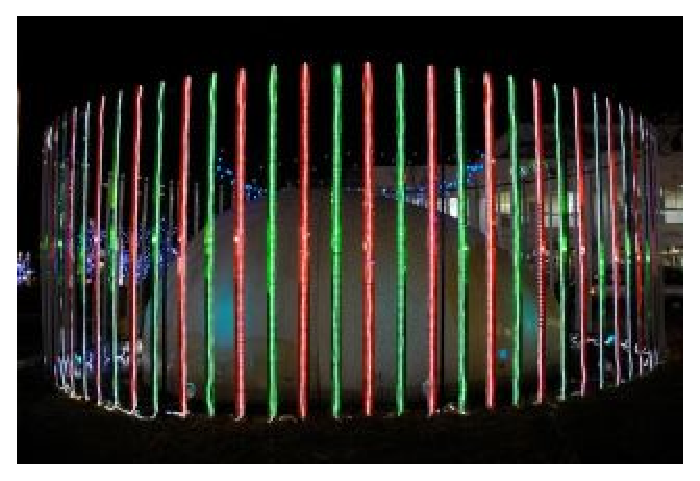
\includegraphics[width=\linewidth]{figs/egg_R.eps}
            			\caption{右目用}
            			\label{fig:egg_R}
                		\end{minipage}
                		\hspace{0.01\linewidth}
                		\begin{minipage}[t]{0.49\linewidth}
            			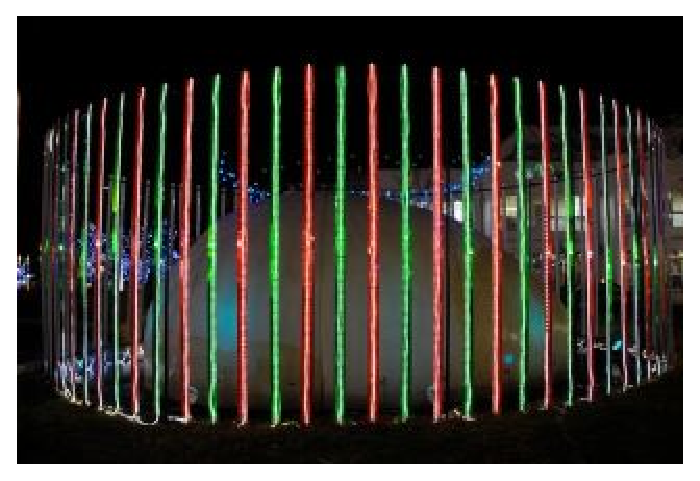
\includegraphics[width=\linewidth]{figs/egg_L.eps}
            			\caption{左目用}
            			\label{fig:egg_L}
        			\end{minipage}
                 \end{figure}
                 
	\item 世界の動物園を巡り、
            	象舍の藁の山の中に卵が隠されていないか、探す。
		これは藁の山の中から針を探すより楽である。

	\item 見通しの効くアフリカのサバンナで、宇宙と地上から象の卵を探す。
		定期的に撮った写真を比較する、超新星探索と同じ画像処理を衛星写真に対して行えば、
		効率的に広範囲の探索ができる。
		象の卵の候補が見つかったら、ハッブル望遠鏡をその方向に向けて写真を撮り、
		現地調査に向かうべきかどうかを判定する。

	\item インドとタイに行き、ジャングルに隠されている卵を探す。
                	ジャングルの場合空からは探しにくいが、象使いも多く、象の背中に乗って
                	象の視点から探索することができる。
                	さらに、気性の荒いアフリカ象と異なり、気だての優しいインド象ならば
                	卵の在処を教えてくれる可能性もある。
		子供時代、象と散歩をした経験があるので\cite{inTheForest}、
		すぐに象と仲良くなれると思う。
		
\end{enumerate}

\vspace*{1zw}
\begin{thebibliography}{99}
	\bibitem{teramura} 寺村輝夫、「ぼくは王様 - ぞうのたまごのたまごやき」.
	\bibitem{inTheForest} マリー・ホール・エッツ、「もりのなか」.
\end{thebibliography}
%end 挑戦的研究の目的及び方法と応募者の研究遂行能力 ====================
% p01_purpose_plan_competence_01.tex
\KLEndSubject{F}


%#Split: 02_importance  
%#PieceName: p02_importance
% p02_importance_00.tex
\KLBeginSubject{02}{2}{2 挑戦的研究としての意義}{1}{F}{}{jsps-subject-header}{jsps-default-header}

\section{2 挑戦的研究としての意義}
%    <<最大 1ページ>>

%s04_importance_chousenteki.tex
%begin 挑戦的研究としての意義 ====================
\vspace*{-8mm}
\subsection{ひらめき}
ある日、風呂につかって温泉卵のことを考えているときに、
世界で一番大きな温泉卵を作るにはどうすればいいかという想いに走り、
世界最大の動物であるシロナガスクジラの卵に思い至った。

\subsection{シロナガスクジラから象へ}
\label{sec:whale}
地球上で最大の生物、シロナガスクジラの卵の研究を進めようとしてきた。
クジラの卵の場合は、高い水圧に耐える必要があるため、堅固の構造となっているはずであり、
これが解明されれば、将来、深海潜水艇への応用も効く。
しかし、シロナガスクジラの生息範囲が広い、海に潜っている時間が長い、
生息数も減っている、などの原因により、
卵を見つけることができなかった。
そこで、\underline{地球で}最大の動物から、
\underline{地上で}最大の動物に研究対象を変更する。
象の卵ならば、はるかに簡単に探索できるはずである。

	この発見により、哺乳類は卵を産まないという学術の世界の
	「常識の殻」を文字通り打ち破ることができる。
	また、他分野の研究の場においても、古くからの「常識の殻」を
	打ち砕くきっかけとなり、科学全体が大きく前進するきっかけとなる。
%end 挑戦的研究としての意義 ====================

% p02_importance_01.tex
\KLEndSubject{V}


%#Split: 03_rights  
%#PieceName: p03_rights
\input{pieces/p03_rights_00}
\section{3 人権の保護及び法令等の遵守への対応}
%    <<最大 1ページ>>

% s09_rights
%begin 人権の保護及び法令等の遵守への対応 ====================
	象の卵のES細胞の培養、象のクローンの生成などは行わない。
	象個体を現地から持ち出すことはないので、ワシントン条約ならびに
        生物多様性条約に抵触しない。また、組換え実験は行なわないので、
        カルタヘナ議定書にも抵触しない。

        \noindent
        \rule{\linewidth}{1pt}
        \linenumbers
        \subsection{ついでに\LaTeX の便利な機能}
        \subsubsection{節}
        通常通り\textbackslash subsection, \textbackslash subsubsectionなどが使えます。
        番号は自動的につきます。
        
        \subsubsection*{番号なし節}
        \textbackslash subsubsection* のように* 付きを使うと、節の番号がつきません。
        
        \subsubsection{コメント文}
        %う〜ん、これ言おうか言わまいか迷てんねんけどな、
        %言うのも何やし、言わへんのもどうかと思うし、どうしようかなあ....
        \LaTeX では当たり前ですが、
        今はとりあえず消すけど使う可能性のある文章は、
        消さずに行の頭に \% をつけてコメントアウトすると、後で復活できます。
        \texttt{TeXShop}や\texttt{TeXWorks}では、複数行選んでまとめてコメントにしたり
        コメントから外したりできます。
        
        \subsubsection{編集用の行番号}
        \texttt{lineno}というパッケージを使えば、
        \textbackslash linenumbersと\textbackslash nolinenumbersの間の行に行番号が振られます。
        これは編集中に他の人からコメントをもらうときに便利です。\\
        \textbf{最終版のPDFを作る前に、行番号は消してください。}
        
        \subsubsection{編集用の欄外のメモ}
        \textbackslash memo{}を使うと右の例のように、欄外にメモを書けます。\\
        \memo{欄外メモ\\だよ}
        \textbf{最終版のPDFを作る前に、\LaTeX ソースファイルの60行目付近にある指示に従って、}
        \textbackslash memo \textbf{を無効化してください。}
        
        \nolinenumbers
%end 人権の保護及び法令等の遵守への対応 ====================

\input{pieces/p03_rights_01}

%#Split: 99_tail
\input{pieces/hook9} % pieces
\end{document}

